\documentclass{estilo}
\usepackage[spanish]{babel}
\usepackage{graphicx}
\usepackage{float}
\usepackage{amsmath}        % para los vectores columnas
\usepackage{amsfonts}       % para las negrita de pizarra
\usepackage{amssymb}        % para simbolos matematicos
\usepackage{hyperref}       % para utilizar referencias
\usepackage{multirow}       % para las tablas
\usepackage{dsfont}
\usepackage{listings}
\usepackage{tikz}
\usetikzlibrary{positioning}
\usetikzlibrary{arrows.meta}
\usepackage{xcolor}
\definecolor{codegreen}{rgb}{0,0.6,0}
\definecolor{codegray}{rgb}{0.5,0.5,0.5}
\definecolor{codepurple}{rgb}{0.58,0,0.82}
\definecolor{backcolour}{rgb}{0.95,0.95,0.92}
\lstdefinestyle{mystyle}{
    backgroundcolor=\color{backcolour},   
    commentstyle=\color{codegreen},
    keywordstyle=\color{magenta},
    numberstyle=\tiny\color{codegray},
    stringstyle=\color{codepurple},
    basicstyle=\ttfamily\footnotesize,
    breakatwhitespace=false,         
    breaklines=true,                 
    captionpos=b,                    
    keepspaces=true,                 
    numbers=left,                    
    numbersep=5pt,                  
    showspaces=false,                
    showstringspaces=false,
    showtabs=false,                  
    tabsize=2
}
\lstset{style=mystyle}

\usepackage{enumitem,multicol,setspace}
\newcounter{subenum}[enumi] % para las multicolumnas
\renewcommand{\thesubenum}{\arabic{subenum}}
\usepackage[nomessages]{fp}
\FPeval\thecolwidth{round(1/4:4)}% Specify number of columns -> column width
\newcommand{\newitem}[1]{%
  \refstepcounter{subenum}%
  \parbox{\dimexpr\thecolwidth\linewidth-.5\columnsep}{%
    \makebox[\labelwidth][r]{(\thesubenum)\hspace*{\labelsep}}%
    #1}\hfill%
}

\usepackage{scalerel,stackengine} % para el sombrero
\stackMath
\newcommand\rhat[1]{%
\savestack{\tmpbox}{\stretchto{%
  \scaleto{%
    \scalerel*[\widthof{\ensuremath{#1}}]{\kern-.6pt\bigwedge\kern-.6pt}%
    {\rule[-\textheight/2]{1ex}{\textheight}}%WIDTH-LIMITED BIG WEDGE
  }{\textheight}% 
}{0.5ex}}%
\stackon[1pt]{#1}{\tmpbox}%
}
\parskip 1ex

\usepackage{mathtools}      % floor y ceil
\DeclarePairedDelimiter\ceil{\lceil}{\rceil}
\DeclarePairedDelimiter\floor{\lfloor}{\rfloor} 

\usepackage[style=authoryear-comp]{biblatex}


\begin{document}
\maketitle

\justifying{}

\newpage
\section{Alcance}

\subsection{Propósito del sistema}
Nuestro sistema de gestión para comedores universitarios busca modernizar la experiencia de estudiantes y personal, permitiendo a los primeros consultar el menú, realizar y pagar pedidos desde la web/dispositivo móvil, y brindando al personal herramientas para gestionar pedidos, preparación en cocina y disponibilidad de productos en tiempo real. Adicionalmente, facilita la administración del menú, stock, promociones y accesos del personal.

\subsection{Alcance funcional}
\subsubsection*{Actores principales}
\begin{itemize}
  \item \textbf{Estudiante}: se registra y autentica, gestiona su perfil, consulta menú y disponibilidad, realiza y paga pedidos, consulta estado y recoge.
  \item \textbf{Personal de cocina/caja}: visualiza pedidos entrantes, cambia estados, gestiona disponibilidad operativa.
  \item \textbf{Encargado/a del comedor}: administra menú, ingredientes, combos/paquetes, stock, promociones, y acceso del personal.
\end{itemize}

\subsubsection*{Funciones incluidas}
\begin{itemize}
  \item \textbf{Gestión de usuarios}: registro con validación de email; autenticación y recuperación de cuenta; perfil con nombre, apellido, email, foto, edad, género y domicilio.
  \item \textbf{Catálogo y composición de productos}:
    \begin{itemize}
      \item Ítems individuales y \emph{combos} (paquetes con precio especial).
      \item Ítems compuestos por ingredientes; dependencia de disponibilidad por ingrediente.
      \item Disponibilidad automática: si falta un ingrediente clave, los ítems/combos afectados quedan \emph{no disponibles} para los estudiantes.
    \end{itemize}
  \item \textbf{Gestión de stock}: alta/baja/ajuste de ingredientes y productos; disparadores para reposición (manual inicialmente).
  \item \textbf{Promociones dinámicas}: reglas configurables (p.ej., ``con un sándwich, un café gratis'', 3x2, descuentos por día o por monto).
  \item \textbf{Ciclo de vida del pedido}:
    \begin{enumerate}
      \item \emph{Confirmado} por el estudiante.
      \item \emph{En preparación} por personal de cocina.
      \item \emph{Listo para retirar}.
      \item \emph{Completado} al momento del retiro.
    \end{enumerate}
    \noindent \emph{Cancelación} permitida mientras no haya comenzado la preparación.
  \item \textbf{Backoffice del encargado}: ABM de menú, ingredientes, combos, promociones y gestión de accesos del personal.
  \item \textbf{Pagos}: registro de pagos asociados al pedido
\end{itemize}

\subsection{Alcance no funcional}
\begin{itemize}
  \item \textbf{Seguridad y autenticación}: autenticación con tokens (JWT), almacenamiento seguro de credenciales.
  \item \textbf{Disponibilidad}: servicio operativo en horario del comedor; tolerancia a picos en horarios pico.
  \item \textbf{Rendimiento}: respuesta rapidas para consultas de menú bajo carga típica; actualización de estados en tiempo real en vistas de cocina/pedidos.
  \item \textbf{Consistencia}: para operaciones críticas (estado del pedido, disponibilidad de ingredientes).
  \item \textbf{Calidad verificable}: cobertura de tests $\geq 80\%$ en backend.
  \item \textbf{Compatibilidad}: API documentada (Swagger/Postman); contenedores Docker para despliegue.
\end{itemize}

\subsection{Stakeholders y usuarios}
\begin{itemize}
  \item \textbf{Estudiantes} (usuarios finales).
  \item \textbf{Personal del comedor} (cocina/caja).
  \item \textbf{Encargado/a del comedor} (administración y configuración).
  \item \textbf{Equipo de TI/desarrollo} (operación y evolución).
\end{itemize}

\subsection{MVP / Early Testable Product}
\label{subsec:mvp}
\begin{itemize}
  \item Registro, autenticación, validación de email y recuperación de contraseña.
  \item Menú con disponibilidad por stock e ingredientes.
  \item Flujo de pedido de extremo a extremo.
  \item Panel de cocina y backoffice mínimos.
  \item Registro de pagos.
  \item API y despliegue en Docker para pruebas.
\end{itemize}

\newpage
\section{Arquitectura de Software}

El sistema a implementar para cumplir con los requisitos funcionales pueden ser
descripto en función de los siguientes:

• Ser accesible a múltiples usuarios.
• Permitir que los usuarios puedan interactuar con el sistema cumpliendo diferentes roles y
garantizar que ciertas funcionalidades estén disponibles sólo para algunos roles.
• Realizar validaciones sobre las operaciones que los usuarios intentan llevar a cabo, de
manera de garantizar el cumplimiento de las reglas de negocio y la consistencia de la
información almacenada.
• Permitir operaciones tanto de actualización como de consulta, de lo cual se deriva que se
debe almacenar el resultado de las operaciones efectuadas en algún medio persistente. 

Se decidió utilizar un patrón de arquitectura Enterprise, vinculado con el patron de layer. Se definieron las siguientes capas:
\begin{itemize}
        \item \textbf{Capa de presentación}: Encargada en presentar la información a los distintos usuario y permitiéndo, a partir de eventos generados por el usuario, interactuar con la capa de servicio.
        \item \textbf{Capa de servicio}: Brinda las funcionalidades necesarias para los distintos casos de uso a la capa de presentación e interactua con la capa de negocio.  
        \item \textbf{Capa de negocio}: Implementa todas las reglas de negocio necesarias para que se cumplan los requisitos pedidos.
        \item \textbf{Capa de persistencia}: Ofrece a la capa de negocio el servicio de persistir, almacenar y recuperar la información.
\end{itemize}
\section{Vista Lógica}

\begin{figure}[H]
    \centering
    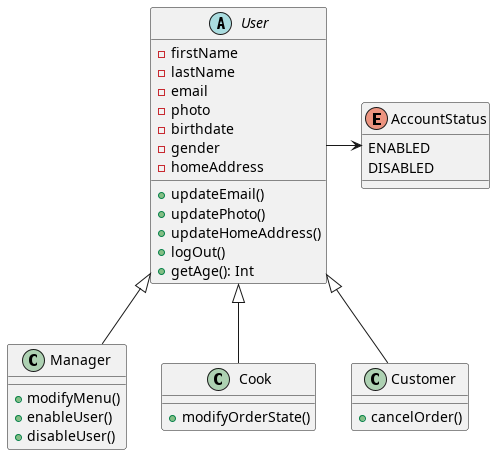
\includegraphics[width=0.5\textwidth]{img/diagrama_de_clases_user}
    \caption{Diagrama de Clases: Usuarios}
    \label{fig:dc1}
\end{figure}

La entidad \texttt{User} representa a cualquier persona que utiliza el sistema
(estudiante/cliente, personal del comedor o encargado). Contiene los datos de
identidad y autenticación (email, contraseña) y se asocia a un único
\texttt{Role}, que indica el tipo de usuario y, por lo tanto, los permisos que
posee. El enum \texttt{Role} distingue entre usuarios administradores
(\texttt{ROLE\_ADMIN}), empleados del comedor (\texttt{ROLE\_EMPLOYEE}) y
clientes finales (\texttt{ROLE\_CLIENT}). A partir de este rol, la capa de
seguridad aplica las políticas de autorización para acceder a los distintos
casos de uso del sistema.


\begin{figure}[H]
    \centering
    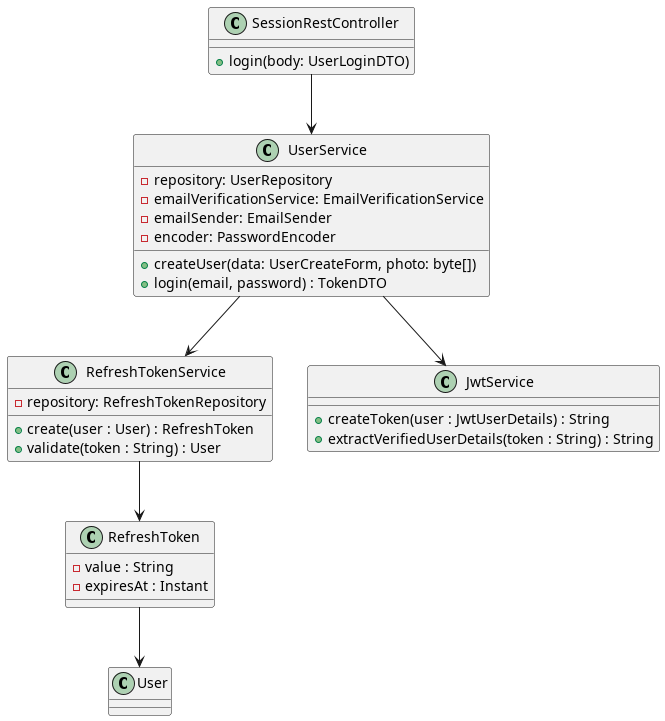
\includegraphics[width=0.7\textwidth]{img/diagrama_de_clases_user_sessions}
    \caption{Diagrama de Clases: Autenticacion de usuarios}
    \label{fig:dc1_auth}
\end{figure}

El subsistema de autenticación se organiza alrededor de \texttt{UserService},
que concentra la lógica de inicio de sesión y refresco de tokens. El
\texttt{SessionRestController} expone los endpoints HTTP de \texttt{login} y
\texttt{refresh} y delega el trabajo en dicho servicio. A partir de las
credenciales recibidas, \texttt{UserService} valida al \texttt{User}, genera
un token de acceso JWT mediante \texttt{JwtService} y un token de refresco
persistido como \texttt{RefreshToken} a través de \texttt{RefreshTokenService},
devolviendo ambos en un \texttt{TokenDTO}. De esta forma, el cliente puede
autenticarse usando JWT y renovar su sesión sin reenviar la contraseña.

\begin{figure}[htbp]
    \centering
    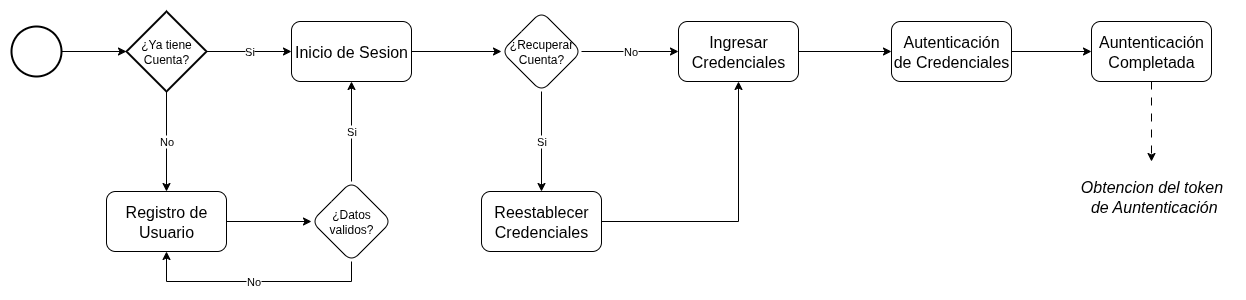
\includegraphics[width=1\textwidth]{img/Diagrama-de-estados-auth}
    \caption{Diagrama de Estados: Autenticacion de un Cliente}
    \label{fig:de2}
\end{figure}

\vfill

\begin{figure}[htbp]
    \centering
    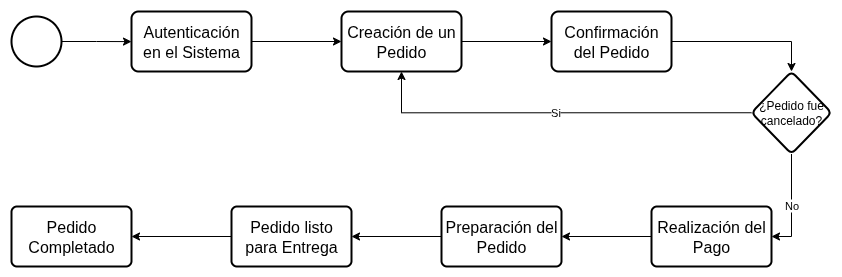
\includegraphics[width=1\textwidth]{img/Diagrama-de-estados-flujo-cliente}
    \caption{Diagrama de Estados: Flujo de un Cliente}
    \label{fig:de1}
\end{figure}

\vfill
\begin{figure}[htbp]
    \centering
    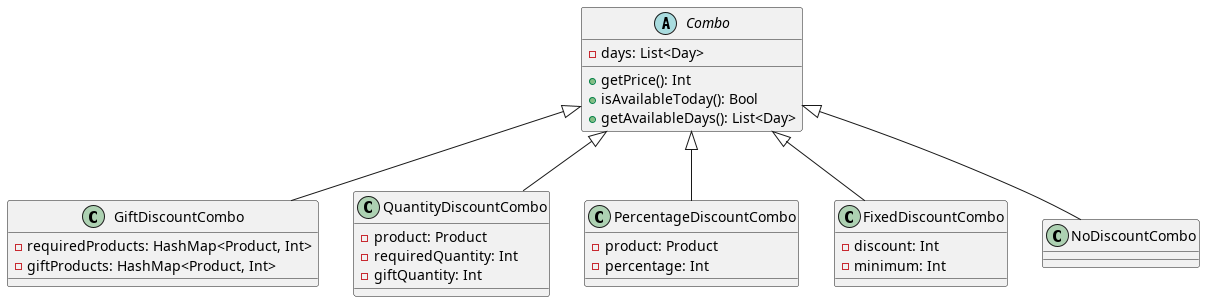
\includegraphics[width=1\textwidth]{img/diagrama_de_clases_productos}
    \caption{Diagrama de Clases: Combos y Productos}
    \label{fig:dc2}
\end{figure}
\vfill

\begin{figure}[H]
    \centering
    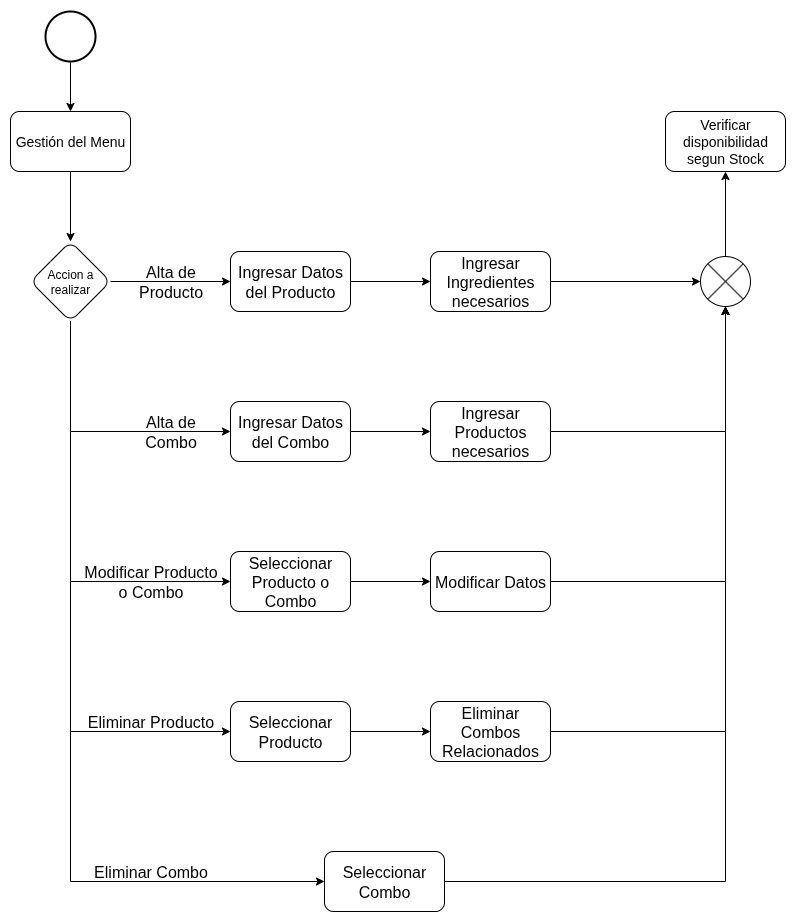
\includegraphics[width=0.7\textwidth]{img/Diagrama-de-estados-productos}
    \caption{Diagrama de Estados: Productos}
    \label{fig:de3}
\end{figure}

El siguiente diagrama modela la lógica de stock y precios del sistema. La interfaz
\texttt{Stockable} abstrae a cualquier elemento cuya disponibilidad pueda consultarse,
mientras que \texttt{Priceable} representa a los elementos que tienen un precio asociado.
\texttt{OrderItem} es una clase abstracta que unifica el comportamiento de los ítems que
pueden formar parte de un pedido (productos y combos), exponiendo operaciones para conocer
su precio, verificar disponibilidad y obtener los ingredientes que consumen. Los
\texttt{Product} se componen de uno o más \texttt{Ingredient}, que son quienes mantienen
el stock físico (\texttt{quantity}), y los \texttt{Combo} se componen de varios
\texttt{Product}. De esta forma, la disponibilidad de productos y combos se calcula siempre
en función del stock real de los ingredientes.

\begin{figure}[H]
    \centering
    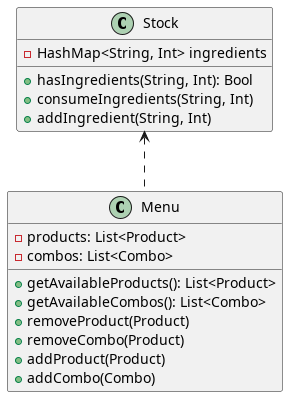
\includegraphics[width=0.4\textwidth]{img/diagrama_de_clases_stock}
    \caption{Diagrama de Clases: Stock}
    \label{fig:dc3}
\end{figure}


\begin{figure}[htbp]
    \centering
    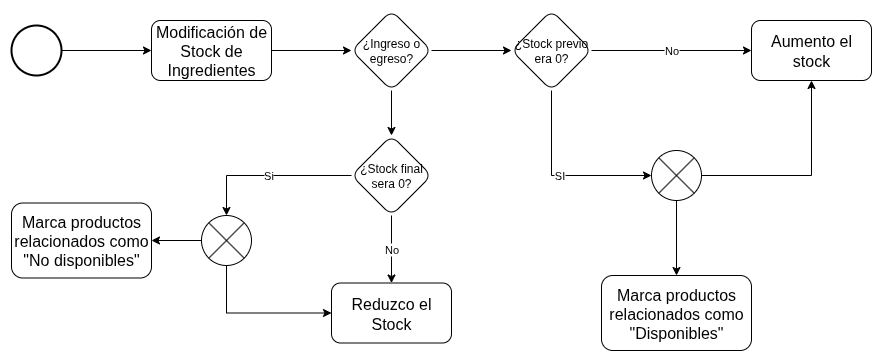
\includegraphics[width=1\textwidth]{img/Diagrama-de-estados-Gestion-de-stock}
    \caption{Diagrama de Estados: Stock}
    \label{fig:de4}
\end{figure}

\vfill
\begin{figure}[htbp]
    \centering
    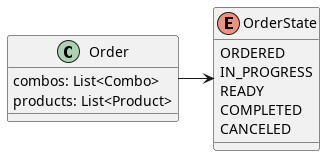
\includegraphics[width=0.4\textwidth]{img/diagrama_de_clases_estado_de_una_orden}
    \caption{Diagrama de Clases: Estados de una Orden}
    \label{fig:dc4}
\end{figure}
\vfill

\newpage

\section{Vista de Procesos}

En la implementación actual se distinguen tres procesos lógicos principales, desplegados
como servicios independientes:

\begin{itemize}
  \item \textbf{Cliente}: el navegador del usuario, donde se ejecuta la aplicación web. Desde aquí se realizan las peticiones HTTP al sistema, tanto para
        cargar la interfaz inicial como para invocar la API (por ejemplo, login, gestión
        de pedidos, consulta de menú, etc.).
  \item \textbf{Servidor de frontend}: servicio web que sirve los recursos
        estáticos de la aplicación (HTML, CSS, JavaScript) y actúa como punto de entrada
        público. Una vez cargada la app web en el navegador, el servidor de frontend sigue
        atendiendo peticiones de recursos estáticos, pero la mayor parte de la
        interacción ocurre entre el cliente y la API backend.
  \item \textbf{Servidor backend}: aplicación Spring Boot que implementa las capas de
        controlador, servicio y persistencia. Expone la API REST que utiliza el cliente
        para todas las operaciones de negocio (usuarios, autenticación, pedidos, menú,
        descuentos, etc.) y se comunica con la base de datos relacional.
\end{itemize}

Adicionalmente existe un proceso de base de datos (PostgreSQL) que persiste el estado
del sistema y que es utilizado exclusivamente por el servidor backend. En el diagrama
se lo representa como un servicio de soporte para simplificar el foco en la interacción
cliente--aplicación.

\begin{figure}[htbp]
          \centering
          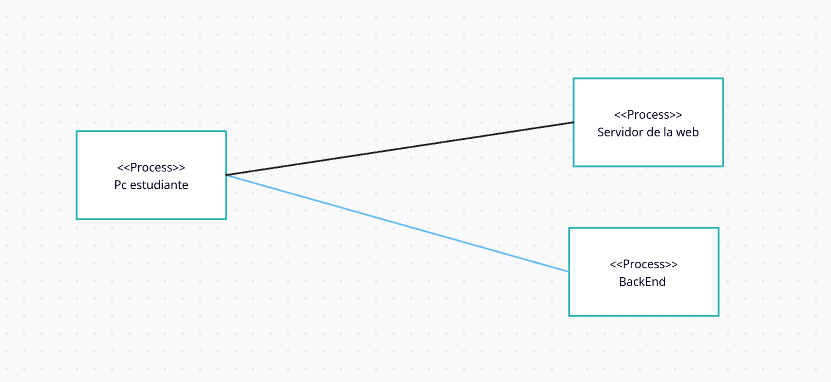
\includegraphics[width=0.9\textwidth]{img/Vista_procesos.png}
          \caption{Diagrama de la vista de procesos}
          \label{fig:mi_imagen}
        \end{figure}

\newpage
\section{Vista de Desarrollo}

En la vista de desarrollo se distinguen dos proyectos principales, que se
corresponden con las carpetas del repositorio:

\begin{itemize}
  \item \textbf{Frontend} (\texttt{frontend/}): aplicación web en React que
        implementa la capa de presentación. Dentro de este proyecto se
        distinguen la UI (páginas y componentes) y los servicios de acceso a
        la API (hooks y funciones de \texttt{apiFetch}).
  \item \textbf{Backend} (\texttt{backend/}): aplicación Spring Boot que
        implementa las capas de aplicación, dominio e infraestructura. Se
        organizan los paquetes de controladores REST, servicios de
        negocio (Aplicación), entidades/agregados (Dominio) y componentes de
        infraestructura (repositorios, seguridad, envío de emails).
\end{itemize}

A nivel conceptual, estos proyectos respetan la separación en capas de
Presentación, Aplicación, Dominio e Infraestructura descrita en la
arquitectura de software.


\begin{figure}[H]
    \centering
    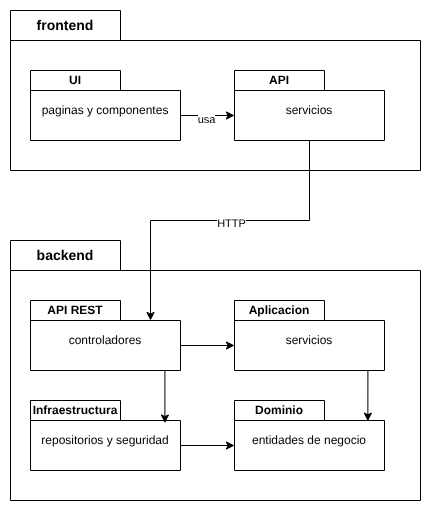
\includegraphics[width=0.6\textwidth]{img/diagrama_de_paquetes}
    \caption{Diagrama de Paquetes}
    \label{fig:dpkg}
\end{figure}

\begin{figure}[H]
    \centering
    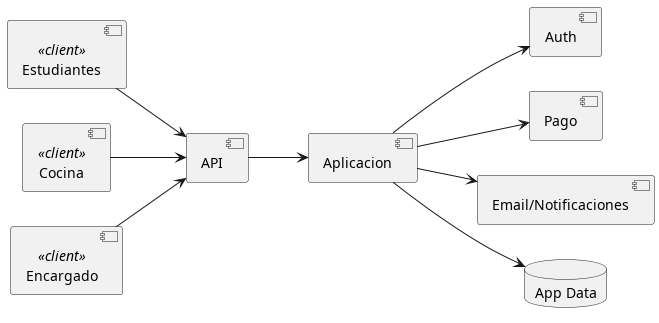
\includegraphics[width=0.6\textwidth]{img/diagrama_componentes}
    \caption{Diagrama de Componentes}
    \label{fig:dcmp}
\end{figure}

El diagrama de componentes muestra la interacción entre la aplicación web
frontend y los componentes principales del backend. El \textbf{Frontend} está
implementado como una SPA en React que ofrece distintas vistas para cliente,
empleado y encargado, y se comunica exclusivamente con la \textbf{API REST} del
backend mediante HTTP.

En el \textbf{Backend} se distinguen los controladores de la API, los
\textbf{servicios de negocio} (pedidos, catálogo, usuarios, descuentos), el
módulo de \textbf{autenticación} basado en JWT y tokens de refresh, y el
módulo de \textbf{email} utilizado para verificación de cuenta y recuperación
de contraseña. Todos estos componentes acceden a la \textbf{base de datos
PostgreSQL} a través de repositorios JPA, donde se persisten usuarios, pedidos,
productos, ingredientes, menús, descuentos y tokens.


\newpage
\section{Vista Física}
Se va a utilizar una arquitectura cliente servidor tipica, en la cual el backend y el acceso a la base de datos van a estar alojados en el mismo servidor y el frontend va a estar alojado en otro.
\begin{figure}[htbp]
          \centering
          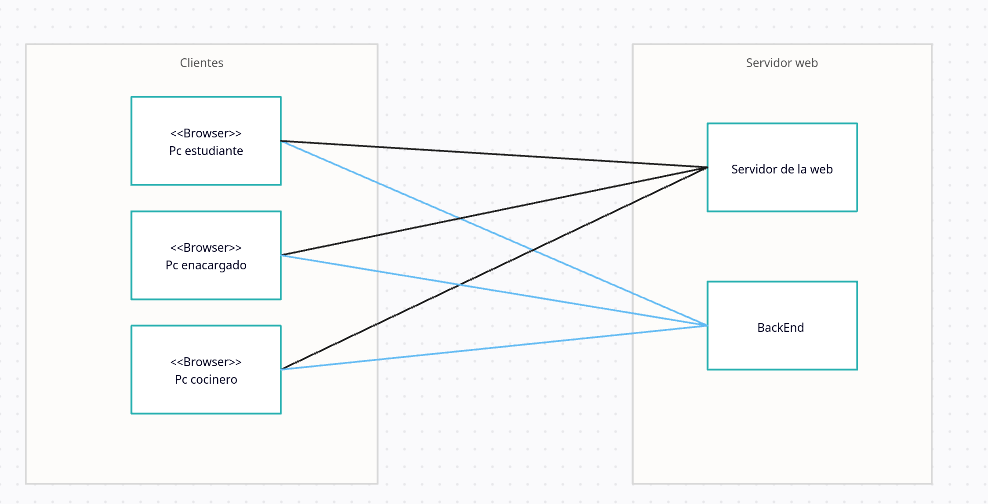
\includegraphics[width=0.9\textwidth]{img/Vista_fisica.png}
          \caption{Diagrama de la vista fisica}
          \label{fig:pysh}
        \end{figure}

En negro se marcaron las conexiones que se dan por primera vez para solicitar la pagina web al servidor. Luego la aplicación se comunicara todo el tiempo con el servidor backend mediante la API de la capa de servicio.

\newpage
\section{Escenarios}

\begin{figure}[htbp]
    \centering
    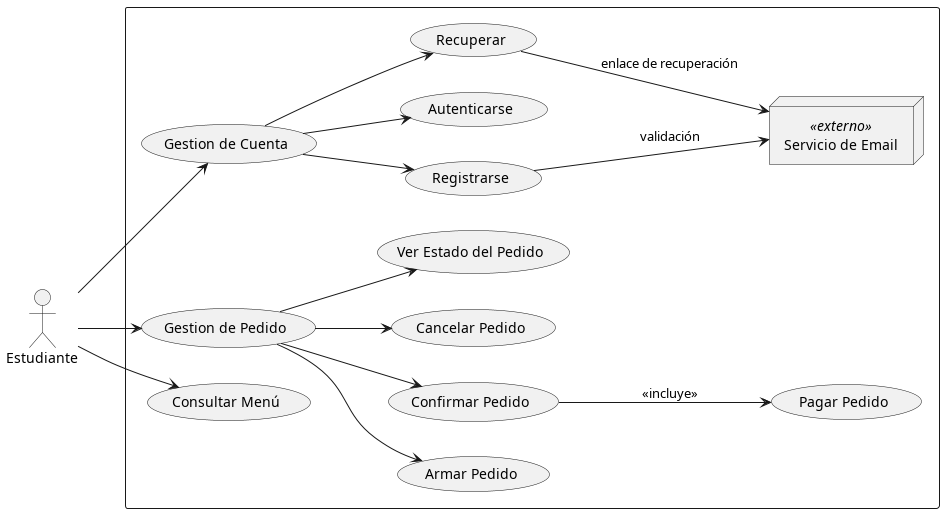
\includegraphics[width=1\textwidth]{img/caso_de_uso_estudiante}
    \caption{Casos de uso: Estudiantes}
    \label{fig:dcu1}
\end{figure}

\vfill
\begin{figure}[htbp]
    \centering
    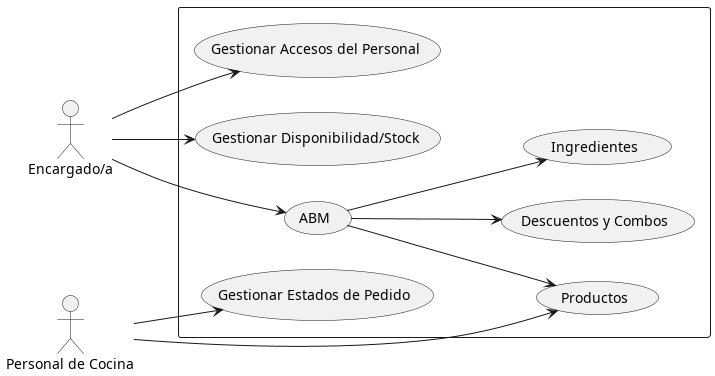
\includegraphics[width=1\textwidth]{img/caso_de_uso_personal}
    \caption{Casos de uso: Personal del comedor}
    \label{fig:dcu2}
\end{figure}
\vfill

\newpage
\end{document}